\documentclass{jsarticle}
\usepackage{diagbox}
\usepackage[dvipdfmx]{graphicx}
\usepackage[T1]{fontenc}
\usepackage{amssymb}
\usepackage{amsmath}
\usepackage{mathtools}
\usepackage{siunitx}
\usepackage{graphics}
\usepackage{enumerate}
\usepackage{here}
\usepackage{multirow}
\usepackage{ulem}
\usepackage{dcolumn}
\usepackage{cases}
\usepackage{textcomp}
\usepackage{siunitx}
\usepackage{here}
\usepackage{float}
\usepackage{array}
\usepackage{multirow}
\usepackage{listings}
\usepackage{url}


\lstset{
    breaklines=true,
    frame=single,
    numbers=left,
    tabsize=2,
    basicstyle=\ttfamily\footnotesize
}

\makeatletter
\@addtoreset{equation}{section}
\def\theequation{\thesection.\arabic{equation}}
\makeatother

\makeatletter % プリアンブルで定義開始

% 表示文字列を"図"から"Figure"へ
\renewcommand{\figurename}{図}

% 図番号を"<章番号>.<図番号>" へ
\renewcommand{\thefigure}{\thesection.\arabic{figure}}

% 章が進むごとに図番号をリセットする
\@addtoreset{figure}{section}

\makeatother % プリアンブルで定義終了

\makeatletter % プリアンブルで定義開始

% 表示文字列を"表"から"Figure"へ
\renewcommand{\tablename}{表}
% 図番号を"<章番号>.<表番号>" へ
\renewcommand{\thetable}{\thesection.\arabic{table}}

% 章が進むごとに表番号をリセットする
\@addtoreset{table}{section}

\makeatother % プリアンブルで定義終了

\makeatletter
	\AtBeginDocument{% リスト番号の付け方
    \renewcommand*{\thelstlisting}{\arabic{section}.\arabic{lstlisting}}
    \renewcommand{\lstlistingname}{コード}
	\@addtoreset{lstlisting}{section}}
\makeatother
\begin{document}

\section{目的}
これまで習ってきたC言語の知識を利用して、比較的大きなプログラムを書くことで、プログラミング言語
の利用方法のまとめを行うと同時に、複雑なアルゴリズムの構築方法を学ぶことを目的とする。

\section{原理}
\subsection{ファイルからの読み込み}
  ファイルの読み込み(または書き込み)には、まずファイルを利用できるようにする「ファイルのオープン」が必要であり、
  コード\ref{c1_1_1}のような形で可能となる。

    \begin{lstlisting}[caption=ファイルからの読み込み1\label{c1_1_1}]
        FILE *file; //  ファイルポインタの定義
        file = fopen("file_name","r"); //  ファイルのオープン r は readの意味
         ( ファイルを使った処理を書く )
        fclose(file);
    \end{lstlisting}

  また、一般的に数値をファイルから読み込むときは、以下のような「fscanf」を利用する。
  フォーマットはコード\ref{c1_1_2}のようであるが、基本的なフォーマットはファイルポインタ
  以外は、scanfと同じである。
  \begin{lstlisting}[caption=ファイルからの読み込み2\label{c1_1_2}]
    fscanf(*file,"\%d",&a);
  \end{lstlisting}

\subsection{配列}
  配列は、同じ名前の(同じ機能を持つ)変数を大量に作成するために用いられる変数である。
  また、配列は"番号"で管理することができ、この番号を出席番号などに対応させて使うこともできる。
  配列の宣言は、コード\ref{c1_2_1}のようになる。
  \begin{lstlisting}[caption=配列の宣言\label{c1_2_1}]
    int a[10];
    float b[10];
  \end{lstlisting}
  ただし、前者の場合、用意される配列はa[0],a[1],......,a[8],a[9]である。
  配列の宣言時は配列の個数を用いて行う、
  宣言によって作成される配列の番号を指定するときは、
  番号-1番の数値を指定する必要がある。その理由は、配列は使用上0番目から格納されるためである。

\subsection{並び替え(ソート)}
  並べ替え(ソート)は、データを大きい順や小さい順に並べることである。逐次比較して、
  並べ替えるようなアルゴリズムは、簡単であるが、時間のかかる方法である。また「クイックソート」
  「バブルソート」などのアルゴリズムは複雑であるが高速となる方法もある。
  \subsubsection{バブルソート}
  バプルソート(bubblesort)の原理は、配列の後ろから先頭に向かってスキャンしていき、
  もし隣り合う2つの要素の大小関係が逆であったら、それを入れ換えるという単純なものである。
  まず最初は、n-1番目(最後)の要素から0番目(先頭)の要素までをスキャンする。
  その結果、最小の要素が0番目(先頭)に浮かび上がっていく。2回目のスキャンでは、
  n-1番目から1番目までの要素をスキャンして、
  結果として次に小さい要素が配列の1番目の位置に浮かび上がってくる。
  さらにスキャンを繰り返していき、最終的にn-1回目のスキャンで整列が完了する。
  整列の過程が、ちょうど軽い要素が浮き上がっていくように見えるため、バブルソート
  (バブル:bubbleとは泡のこと)と呼ばれている\cite{sort}。
  \subsubsection{クイックソート}
  クイックソート(quick. sort)の原理は、
  クイックソートの計算量は0(nlogn)で、n個の要素a[O],a[1] ,...,a[n-1]をもった配列aを整列することを考える。
  まず、ある適当な要素xを1個選び出し、それを最終的に置かれるべき位置a[v]に移動する。
  この要素xを枢軸(pivot)と呼びます。このとき同時に、xより大きな要素はa[v]より右に、
  xより小さな要素はa[v]より左へと振り分けを行います。この操作によって、配列aを次の3つの部分
  (1) a[v]よりも小さい要素、a[O], a[1],...,a[v-1] (2)a[v] (3)a[v]よりも大きな要素a[v+l],a[v+2],...,a[n-l]
  にわけられる。

  a[v]は最終的な位置に移動されていて,そのIt a[v]より小さい要素のみが、その右にはa[v]より大きな要素のみが存在
  するので、2つの部分配列(1)と(3)をそれぞれ別個に整列すれば、配列a全体の整列が完了する。
  部分配列がただ1つの要素になるまで、この分割を繰り返す。

  このように、大きな問題を複数の小さな問題に分割して確固撃破すると言うアプローチは、
  分割統治(divide and rule または divid and conquer)と呼ばれる\cite{sort}。


  \subsubsection{ソートの安定性について}
  ソートの安定性とは、あるデータをソートした時に、元の順番を保持するか、保持しないかである。
  ソートは上記のソート意外にも種類がたくさんあり、それらのソートも含めたソートの安定性についての表を
  表\ref{t1}に示す。

    \begin{table}[htbp]
        \begin{center}
          \caption{ソートの安定性}
            \label{t1}
            \begin{tabular}{c|c}
                安定であるソート & 安定でないソート  \\ \hline
                バブルソート   & シェルソート     \\
                挿入ソート    & ヒープソート      \\
                マージソート   & 選択ソート      \\
                &クイックソート \\
                \end{tabular}
        \end{center}
    \end{table}

\subsection{ファイルへの書き出し}
一般的に数値をファイルヘ書き込む時はまず読み込みと同様にファイルのオープンをしてから(ただし、"r"を、"w"はwriteの意味)、
以下のような「fprintf」を利用する。フォーマットはコード\ref{c1_4_1}のようであるが、
基本的なフォーマットはファイルポインタ以外はprintfと同じである。

 \begin{lstlisting}[caption=ファイルへの書き込み\label{c1_4_1}]
   fprintf(*file, "\%d",a)
 \end{lstlisting}

\subsection{表計算ソフトからの読み込み表計算ソフトへの書き出し}
エクセルやLibreOfficeのCaleなどの表計算ソフトは、保存されているデータを10 20 30 や
「10,20,30」など、C言語で簡単に読み込めるような、数値をスペースやカンマで区切るような形式に変換して保存することができる。
また、C言語で同様の形式でデータをファイルに書き込めば、表計算ソフトで読み込むことができる。
これらを使い、表計算ソフトにあるデータをプログラミング言語で複雑な計算をし、それを表計算ソフトに改めて
読み込ませてグラフ化をする、というようなことができる。

\subsection{構造体}
構造体(structure)は、異なる型をもつデータをひとまとめにしたものである。
配列は、同じ型のデータを集めたものなのに対して、構造体は異なる型のデータを集めた
ものである。構造体というのは、C言語特有の呼び方で、一般の用語ではレコード構造と呼ばれる\cite{sort}。

\newpage
\section{設計}
本実験では、品川高専入試プログラムを作成することを最終の目標とする。
そのプログラムの仕様、設計を以下に示す。
\subsection{仕様}\label{s3_2}
本実験で作成するプログラムの仕様を以下に示す。
\begin{enumerate}
  \item 受験時の国語の点数、数学の点数、英語の点数(100点満点)
  \item 中学校3年次2学期の国語、社会、数学、理科、音楽、美術、保健・体育、技術・家庭、英語の成績
\end{enumerate}

これらのデータ(ファイルに入っている)を使い、成績処理及び順位付けをするプログラムを作成する。
作成には次のような行程を踏んで行う。

\begin{enumerate}
  \item 成績が入ってるファイルから読み込を行い、そのまま処理結果ファイルに保存する。
  \item それぞれの教科の点数を相当する変数に入れる。ただし、配列の添字と受験番号及び、
  教科に対応させる。
  \item 単純に受験時の点の合計をを素点にいれ、中学校の成績の点をそれぞれ総合して、記録点として代入する。
  \item 数学と理科の成績を1.4倍して、それらを使った中学校の成績の点を使って、中学校の成績の合計点
  の最高点の最高点(7点 $\times$ 2教科 $+$ 5教科 $\times$ 5教科 \= 49点)を700点に換算(すなわち中学校の成績の合計点の最高点)
  した値を記録換算点に入れる。
  \item 全ての総合点の平均をとり、平均点以上の受験生に対して合否に1を平均未満の受験生に対しては、0を入力する。
  \item 総合点を高い順番でソート(並べ替え)をファイル「sort.dat」に保存する。ただし、誰がどの点数だったかを記録しておく必要はない。
  \item 総合点を使って、受験生の順位を決定し、順位に代入する。ただし、同点の場合は受験番号が若い(小さい)ものを上位とする。
  \item 処理結果ファイルを使い、受験番号を入力したらその受験生の成績を表示するプログラムを作成する。
\end{enumerate}

\begin{figure}[H]
  \begin{center}
    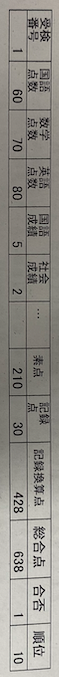
\includegraphics[width = 14cm,angle=90,height=1cm]{f1.png}
    \caption{成績の一例\label{f1}}
  \end{center}
\end{figure}

% \begin{table}[htbp]
%     \begin{center}
%       \caption{成績の一例}
%         \label{t2_1}
%         \begin{tabular}{c|c|c|c|c|c|c|c|c|c|c|c|c}
%             受験番号 &国語点数 & 数学点数 & 英語点数 &国語成績& 社会成績 & その他7科目 &素点&記録点&記録換算点&総合点&合否&順位  \\ \hline
%             1 & 60 & 70 & 80 & 5 & 5 & ... & 210 & 30 & 428 & 638 & 1 & 10    \\
%             \end{tabular}
%     \end{center}
% \end{table}
\newpage
\subsection{入試プログラムの設計}\label{s4_2}
品川高専入試プログラムを作成する時に、
ファイルからの読み込み、内部処理の設計、ソート、ファイルへの書き出し、
表計算ソフトでの読み込みファイルの作成、表計算ソフトでの書き出しファイルの作成、
それらの段階ごとの設計について以下に示す。

\subsubsection{ファイルからの書き込み}
入試プログラムを作成するにあたり、入試テストの元のデータを読み取る必要がある、その機構の設計を以下に示す。
ファイルからの書き込みに用いるファイルとして、可用性の高い、csvファイルからデータを読み取る
プログラムを設計することとした。
入試プログラムに用いるファイルの読み込みは、c言語の標準的な書き込みを用いる。
まずfpというファイルポインタを定義し、前もって、空の配列を宣言しておく。
fpというFILEポインタから一時的に、csvの行の要素を配列の各要素として取り込み、
構造体配列の各メンバに対して、それらの配列を代入することで、ファイルの読み取り処理を行う。

\subsubsection{ソート}
入試プログラムによって計算を行ったあと、得られた数値を高い順に並び替える必要がある、その機構の設計を以下に示す。
テストの得点を降順にソートする。
仕様にある通り、順位が同点の場合、出席番号が若いものを優先する必要がある。
そのため、安定性のあるソートを使う必要があるもしくは、若い番号を優先するように作り替える必要があるため、
今回は前者の安定性のあるソートによって実装することで、仕様に従った。安定性のあるソートは、実装も簡単に行える
バブルソートを採用する。

\subsubsection{ファイルへの書き出し}
入試プログラムを作成するにあたり、読み込みこんだファイルを計算したあと、ファイルを書き出す必要がある、その機構の設計を以下に示す。
ファイルからの書き出しは、ファイルからの読み込みと同等にあらたなファイルポインタfp\_outを作成し、csvファイルの形式で出力を行う。
fprintfを用いて、一行目は各列のラベルを出力する。
また、2行目以降は、構造体配列の要素をfor文をもちいて、構造体配列の各要素を出力する。
各構造体配列ごとに順位を割り振っていき順位も出力する。

\subsubsection{読み込みファイルの表計算ソフトでの作成}
入試プログラムを作成するにあたり、誰でもこのプログラムを使用できるように、
表計算ソフトから読み込みようのファイルを作成することができるようにする必要がある、その設計を以下に示す。
表計算ソフトの保存方法をcsv形式で保存させることで、プログラムからの読み込みを可能にする。

\subsubsection{書き出しファイルの表計算ソフトでの読み取り}
入試プログラムを作成するにあたり、誰でもこのプログラムを使用できるように、
表計算ソフトによって、プログラムで出力されたファイルを閲覧できるようにする必要がある、その設計を以下に示す。
プログラムによって出力されるファイルをcsvファイルとすることによって、閲覧を可能にする。

\subsubsection{処理結果のグラフ化}
表計算ソフトで出力されたデータのみでは、そのテスト事態の傾向や、その年の点数の分布を視覚的にわかりやすいとは言えない。
そのため、表計算ソフトを用いて処理結果をグラフ化する。その設計を以下に示す。
総合点の最大値は1000点であるため、階級値を100刻みの数値として、度数分布表を作成する。

\newpage
\section{実装}
\subsection{実装環境}
実装に用いた環境の情報を\ref{t2}に示す。
\begin{table}[htbp]
            \begin{center}
              \caption{実験環境}
                \label{t2}
                \begin{tabular}{l||c|c}
                    ツール & ツール名 & バージョン\\ \hline
                    プログラミング言語 & c & Apple clang version 12.0.5 (clang-1205.0.22.9)\\
                    OS & Mac OS Big Sur & 11.2.3\\
                    CPU & Intel Core i5 & 2 GHz クアッドコア \\
                    メモリ & LPDDR4X & 16 GB 3733 MHz  \\
                    表計算ソフト&Micro Soft Excel & 16.48\\
                    \end{tabular}
            \end{center}
        \end{table}

\subsection{実装したプログラム}
設計を元にして本実験で最終的に実装した入試プログラムを\ref{c4_1}に示す。
\begin{lstlisting}[caption=成績処理のプログラム\label{c4_1}]
  #include <stdio.h>
  #include <stdlib.h>
  #include <string.h>
  #define NUM 13
     struct score {
      int number; //  受験番号
      int japanese_score; //  国語のテスト点
      int math_score; // 数学のテスト点
      int english_score; // 英語のテスト点

      int japanese_grade; // 国語の成績
      int ss_grade; //  社会の成績(social studies)
      int math_grade; // 数学の成績
      int science_grade; // 理科の成績
      int music_grade; // 音楽の成績
      int art_grade; // 美術の成績
      int pe_grade; // 体育の成績
      int helt_grade; // 技術家庭 (home economics life technique)
      int english_grade; // 英語の成績

      int total_score; // テスト点数の合計
      int total_grade; // 内申点の合計
      float base_score; // 記録換算点(内申点を点数化したもの)

      float score; // 全てを考慮した点数

      int result; // 合否
      int rank; // 順位
    };

  void score_sort(struct score scores[],int ninzu){
     int s,t;
     struct score tmp;
      for(s=0 ; s<ninzu-1 ; s++){
          for(t=s+1;t<ninzu;t++){
              if(scores[t].score>scores[s].score){
                  tmp = scores[t];
                  scores[t] = scores[s];
                  scores[s] = tmp;
                  // bubble sort sort の安定性が高いため採用
              }
          }
      }
  }

  int avg_score(struct score scores[],int ninzu){
    int i;
    float avg;
    for(i=0;i<ninzu;i++){
      avg += scores[i].score;
    }
    avg = avg/i;
    return avg;
  }

  int main(){
    FILE *fp;
    FILE *fp_out;

    char *fname = "input.csv";
    int ret , i=0 ,avg;
    char buf[NUM][100];
    int data[NUM];
    char fname_out[24];

    // ファイルを開く
    fp = fopen( fname, "r" );
    if( fp == NULL ){
      printf( "%sファイルが開けません\n", fname );
      return -1;
    }


    fscanf(fp, "%[^,],%[^,],%[^,],%[^,],%[^,],%[^,],%[^,],%[^,],%[^,],%[^,],%[^,],%[^,],%s",
    buf[0], buf[1], buf[2], buf[3],buf[4],buf[5],buf[6],buf[7],buf[8],buf[9],buf[10],buf[11],buf[12]);

    struct score scores[500];

    while((ret=fscanf(fp, "%d, %d, %d, %d, %d, %d, %d, %d, %d, %d, %d, %d ,%d",
    &data[0], &data[1], &data[2], &data[3], &data[4], &data[5], &data[6],
    &data[7], &data[8], &data[9], &data[10], &data[11], &data[12])) != EOF){
      scores[i].number =data[0];
      scores[i].japanese_score =data[1];
      scores[i].math_score = data[2];
      scores[i].english_score =data[3];

      scores[i].japanese_grade =data[4];
      scores[i].ss_grade =data[5];
      scores[i].math_grade =data[6];
      scores[i].science_grade =data[7];
      scores[i].music_grade =data[8];
      scores[i].art_grade =data[9];
      scores[i].pe_grade =data[10];
      scores[i].helt_grade =data[11];
      scores[i].english_grade =data[12];

      scores[i].total_score = data[1]+data[2]+data[3];
      scores[i].total_grade =data[4]+data[5]+data[6]+data[7]+data[8]+data[9]+data[10]+data[11]+data[12];
      scores[i].base_score =700*((data[4]+data[5]+(data[6]*1.4)+data[7]+data[8]+data[9]+data[10]+data[11]+(data[12]*1.4))/49);

      scores[i].score = scores[i].total_score + scores[i].base_score;
      ++i;
    }

    int ninzu = i;

    avg = avg_score(scores,ninzu);
    score_sort(scores,ninzu);

    // ファイル出力
    int year = 2021 ,month = 4;
    sprintf( fname_out, "%04d%02dresult.csv", year, month);

    //  ファイルのオープン
    if( (fp_out = fopen( fname_out, "w" )) == NULL ) {
        printf( "結果ファイルがオープンできませんでした\n");
        exit( 1 );
    }

    //  ヘッダ行を出力する
    fprintf( fp_out,
    "number , japanese_score , math_score,English_score, japanese_grade,ss_grade,math_grade, science_grade, music_grade , art_grade , pe_grade , helt_grade, english_grade , total_score , total_grade , base_score, score , result,rank\n"
    );

    //   各データをカンマ区切りで出力する
     for( i = 0; i < ninzu; i++ ) {
       if(scores[i].score>=avg){
           scores[i].result = 1;
       }else{
           scores[i].result = 0;
       }
          scores[i].rank = i+1;

         fprintf( fp_out, "%d,%d,%d,%d,%d,%d,%d,%d,%d,%d,%d,%d,%d,%d,%d,%4.0f,%4.0f,%d,%d\n",
           scores[i].number,
           scores[i].japanese_score,
           scores[i].math_score,
           scores[i].english_score,
           scores[i].japanese_grade,
           scores[i].ss_grade,
           scores[i].math_grade,
           scores[i].science_grade,
           scores[i].music_grade,
           scores[i].art_grade,
           scores[i].pe_grade,
           scores[i].helt_grade,
           scores[i].english_grade,
           scores[i].total_score,
           scores[i].total_grade,
           scores[i].base_score,
           scores[i].score,
           scores[i].result,
           scores[i].rank
           );
     }

    printf( "%s に結果が出力されました\n", fname_out );

    printf("%d",avg_score(scores,ninzu));
    fclose( fp_out );
  }
\end{lstlisting}

\newpage
\section{結果}
実装したプログラムの実行結果を以下に示す。
成績の計算が行われる前の表計算ソフトを使用して作成したcsvファイルを\ref{f2}に示す。

\begin{figure}[H]
  \begin{center}
    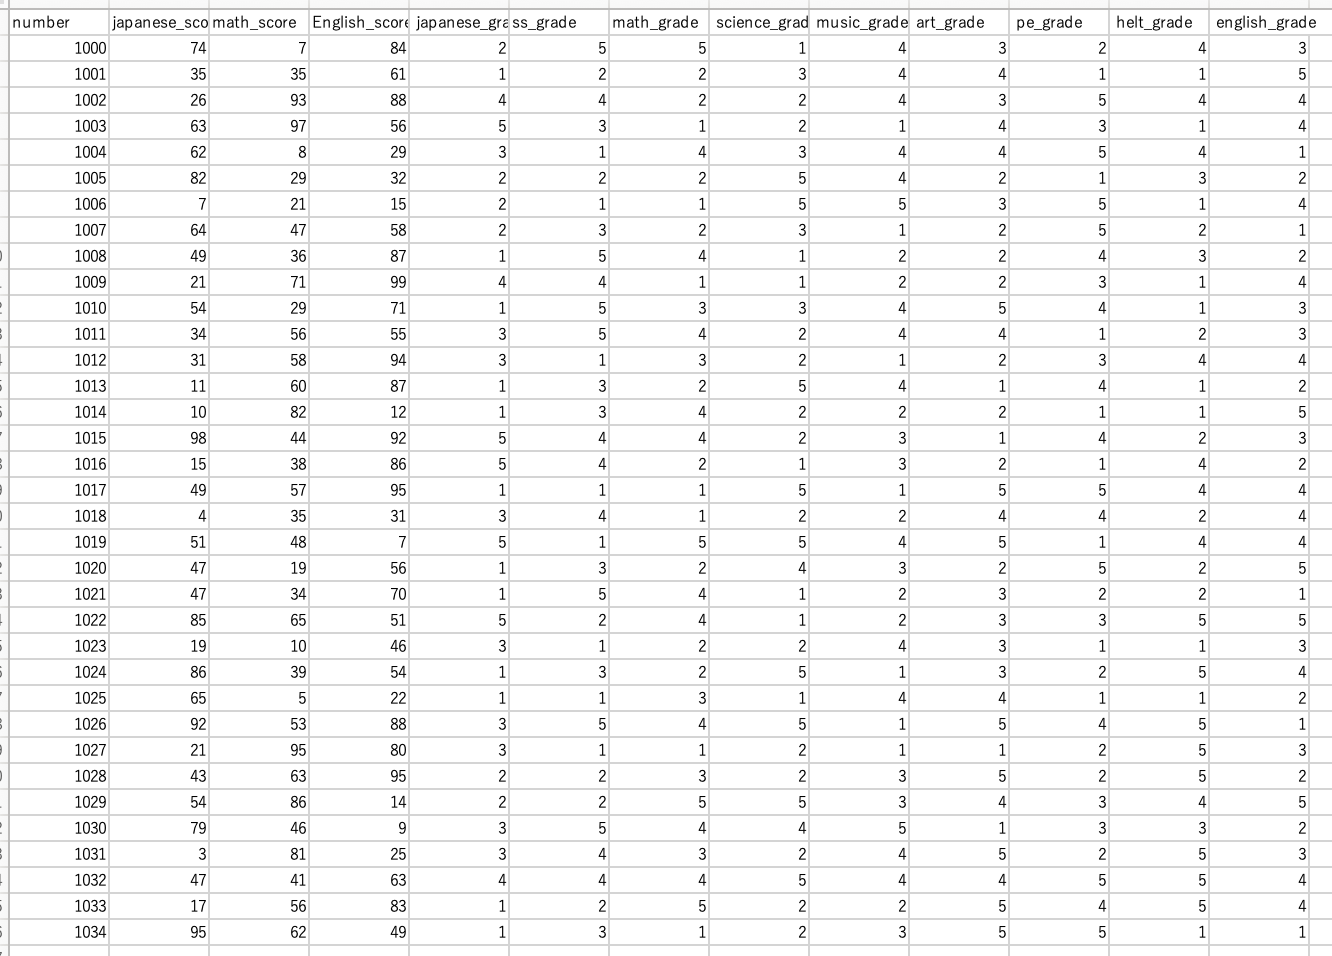
\includegraphics[width = 14cm]{f2-1.png}
    \caption{プログラムが実行される前のcsvファイル\label{f2}}
  \end{center}
\end{figure}

図\ref{f2}のcsvファイルをプログラムを実行し、計算の処理を行った。
処理された後のcsvファイルを図\ref{f3}に示す。

\begin{figure}[H]
  \begin{center}
    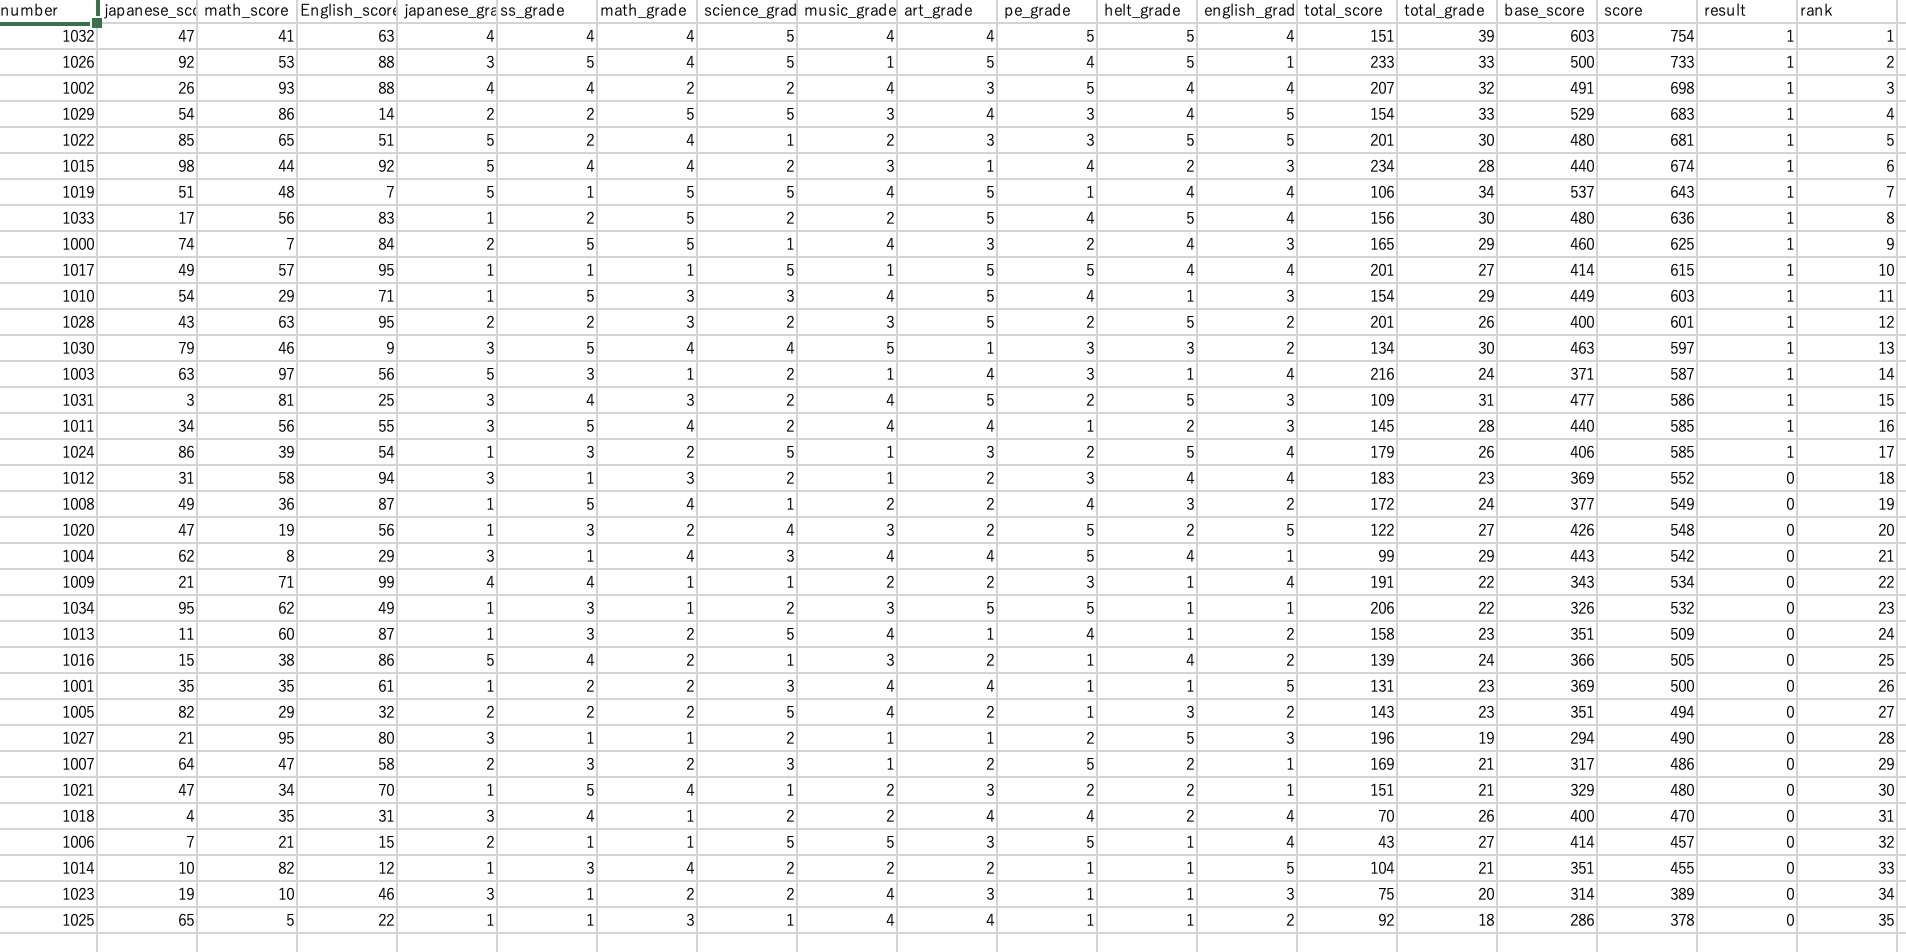
\includegraphics[width = 14cm]{f2.png}
    \caption{プログラムが実行された後のcsvファイル\label{f3}}
  \end{center}
\end{figure}

図\ref{f3}から、
各行で素点、記録点、換算記録点、総合点が出力されていることがわかる。
総合点(score)の平均点を求めた。平均点564.45点
より高い総合点を取っている行の結果(result)は1になっていること、総合点が低い行の結果が0になっていることが確認できた。
また、その総合点の上位から順位が振られていることがわかった。

また、図\ref{f3}を元にして度数分布表を作成した。
その結果を図\ref{f4}に示す。

\begin{figure}[H]
  \begin{center}
    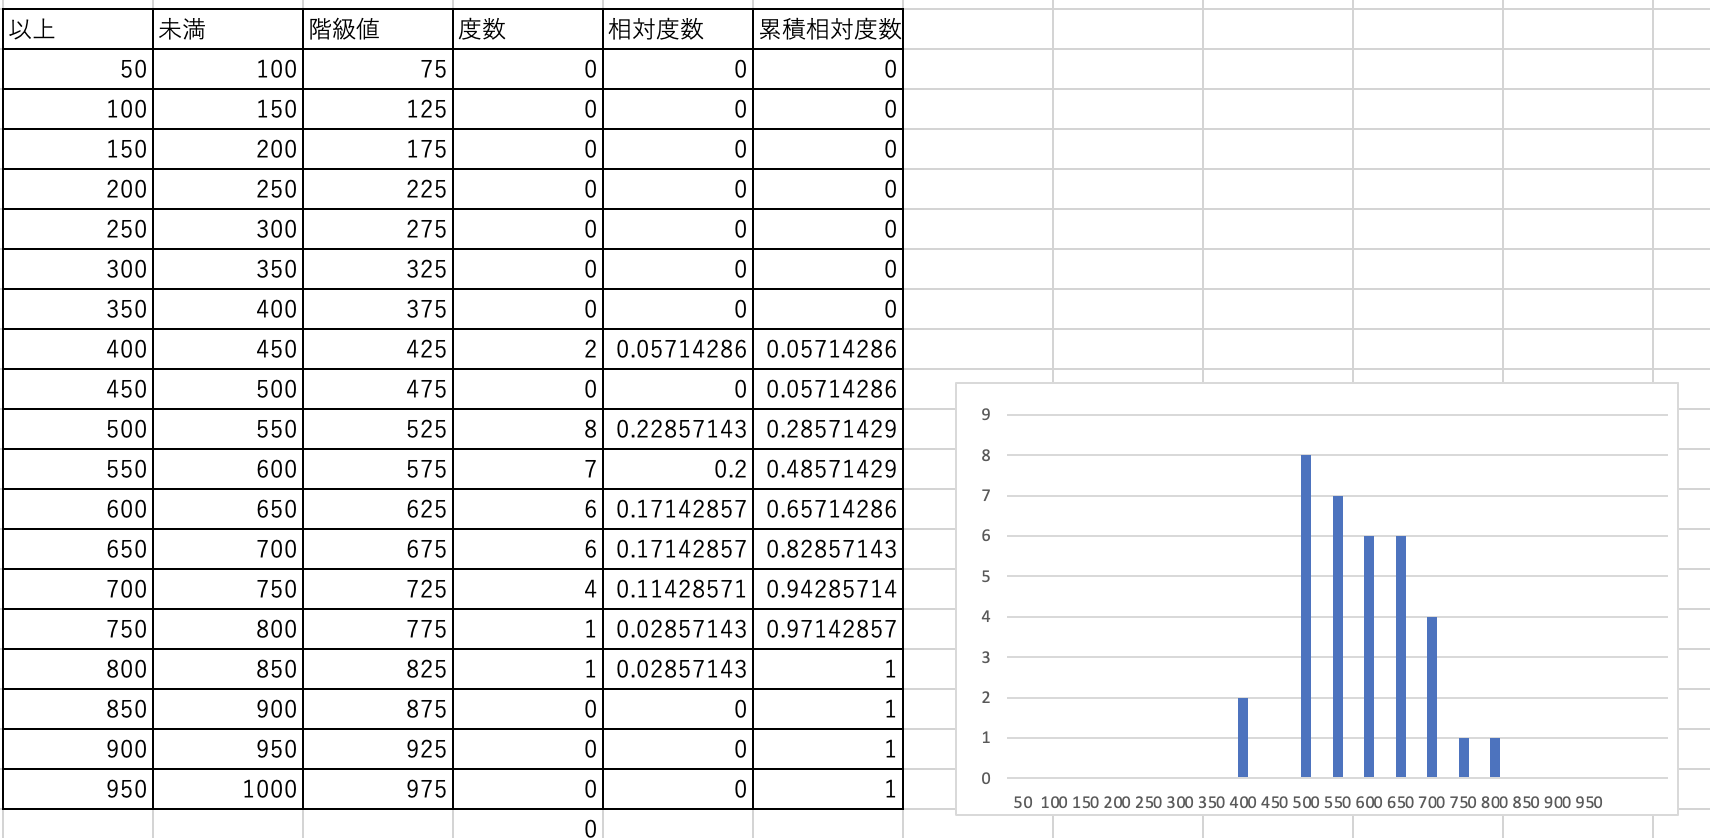
\includegraphics[width = 14cm]{f4.png}
    \caption{図\ref{f3}を元にして作成した度数分布表とヒストグラム\label{f4}}
  \end{center}
\end{figure}


\newpage
\section{考察}
\subsection{構造体の採用について}

本プログラムでは、各生徒の点数を扱うときに、配列ではなく構造体を用いて計算を行った。
構造体を用いるメリットとして、扱っているデータに名前をつけることができるため、
プログラムの可読性が向上する、直感的にデータを操作できることなどの点が挙げられた。
デメリットとして、構造体のデータを他の関数などに渡すときに、構造体をひとまとめで渡す必要があることなどが挙げられた。
上記のメリット、デメリットを加味し、プログラム上で扱う数値が、テストの点数3つ、成績の評定が9つ存在するため、
点数や、評定をみたときに、なんの科目の数値を扱っているのかがわかりやすくするために、
今回実装したプログラムでは、配列ではなく構造体を利用した。
また、上記のことから本実験で実装する際には構造体を用いた方が実装が容易であることが考えられる。

\subsection{バブルソートの採用について}
設計においても示した通り、ソートを実装する際に、バブルソートを用いて、実装を行った。
バブルソートはソートの安定性があるソートなので、総合点が同じ行が二つ以上あった場合、
点数が若い方が優先されるようになっている。図\ref{f3}の585点の生徒をみてわかるように、
番号が若い方が順位が高くなっていることがわかった。また、バブルソートの計算量はO($N^2$)
であるため、Nの数がさらに増えたときに実行の速度が遅くなることが考えられる。
しかし、実装に対するコストが低くすむこと、高専の入試プログラムとして扱う場合はテストの受験者が多くとも500人
前後であること、を考えると、さほど差はないように考えられる。
もし、このプログラムを統一テストであったり、センター試験のテストであったり、
より複雑な計算をしたりする場合がある時は、マージソートやより早いソートアルゴリズムを採用した方が
より良いプログラムになると考えられる。

\subsubsection{度数分布表について}
表計算ソフトを用いて、度数分布表を作成した。
中央の値に対して山なりなグラフになっていることから、このグラフは正規分布であると言える。
その理由として、テストの点数3つ、成績9つの数値を乱数を用いて生成しているため、であると考えられる。
\newpage
\section{結論}
これまで習ってきたC言語の知識を利用して、比較的大きなプログラムを書くことで、プログラミング言語
の利用方法のまとめを行うと同時に、複雑なアルゴリズムの構築方法を学ぶことができた。

\begin{thebibliography}{99}

      \bibitem{sort} 近藤嘉雪.2018.定本 Cプログラマのためのアルゴリズムとデータ構造.SBクリエイティブ株式会社.
  \end{thebibliography}

\end{document}
